\documentclass[letterpaper,11pt]{article}

% \usepackage{newtxtext} % Use Times text font
% \usepackage{newtxmath} % loads Times-like text and CM math by default % Use Computer Modern math font
\usepackage[margin=1in]{geometry} % Set 1-inch margins all around

% Optional: Better spacing and font rendering
\usepackage[T1]{fontenc}
\usepackage[utf8]{inputenc}
\usepackage{microtype,booktabs,graphicx}
\usepackage[colorlinks,allcolors=blue]{hyperref}       % hyperlinks
\usepackage{multirow}
\usepackage{doi}
\usepackage{color,soul}
\usepackage[font=small]{caption}  % small captions
\usepackage[version=4]{mhchem}
% \usepackage{lscape}
% \usepackage{tabularx} % allows column type X to fill textwidth \begin{tabularx}{\textwidth}{l|c|X}
\usepackage{xltabular}

\usepackage{fancyhdr}
    \pagestyle{fancy}
    \fancyhead[L]{OpenMC Scoping}
    \fancyhead[R]{05 June 2026}
    \fancyfoot[C]{\thepage}
    \renewcommand{\headrulewidth}{0pt} % set to 0 pt to remove header line
    %\renewcommand{\footrulewidth}{XXpt}

\usepackage{titlesec} % Change size and spacing of section titles
\titleformat{\section}{\large\bfseries}{\thesection.}{0.5em}{}
\titlespacing*{\section}{0pt}{0.5ex}{0.5ex}
\titleformat{\subsection}{\normalsize\bfseries}{\thesubsection.}{0.5em}{}
\titlespacing*{\subsection}{0pt}{0.5ex}{0.4ex}
% before, after, and right margin (the starred version suppresses the paragraph indent)

\usepackage{enumitem} % customize 'itemize' margin
\setlist[itemize]{leftmargin=0.5cm, topsep=0pt, partopsep=0pt, itemsep=0pt, parsep=0pt}
\setlist[enumerate]{leftmargin=1cm, topsep=0pt, partopsep=0pt, itemsep=0pt, parsep=4pt}

\setlength{\parskip}{12pt} % 1ex plus 0.5ex minus 0.2ex}
\setlength{\parindent}{0pt}
\setlength{\belowcaptionskip}{0pt} % Space between caption and \toprule

\begin{document}

{\begin{center}
\textbf{\large{Preliminary OpenMC Scoping}}
\end{center}
}
\vspace{-1 em}

Here, we use a low-resolution OpenMC model of Excalibur to get first-order estimates of uranium reaction rates and thus scope the quantity of materials necessary.

\begin{figure}[h]
    \centering
    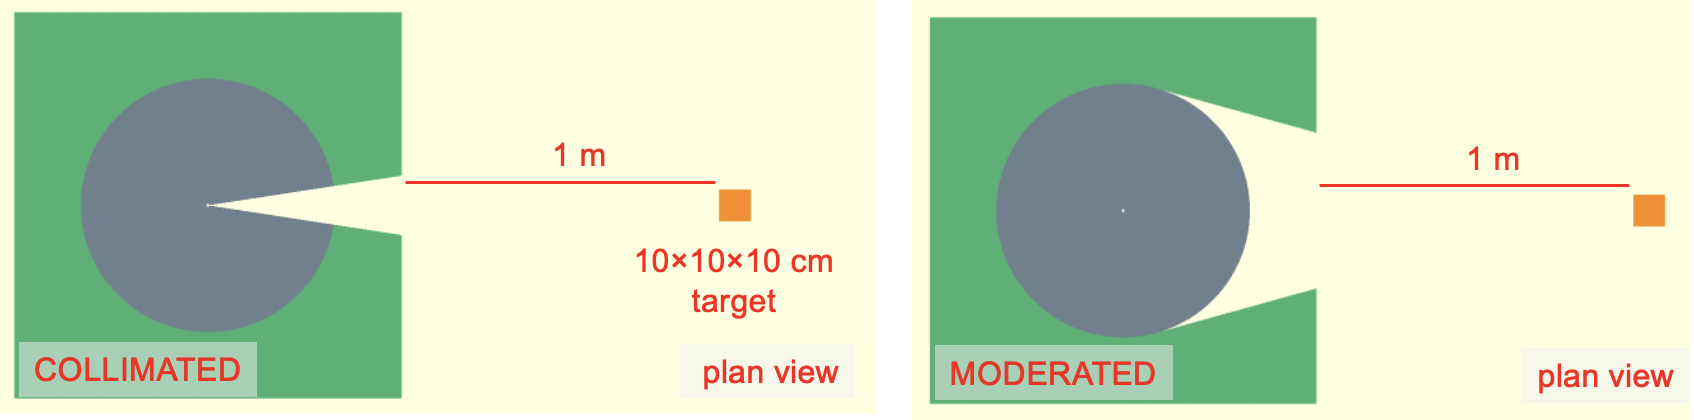
\includegraphics[width=\linewidth]{figs/fig_openmc.png}
    \label{fig:xs}
\end{figure}

{\small
\begin{xltabular}{\textwidth}{l|c|c|ccc|ccc}
    \caption{Uranium reaction rates are generally low.} \\
\toprule
 & \textbf{Target} & \textbf{UX} & \multicolumn{3}{c|}{$\Sigma_\gamma$ \textbf{[1/cm]}} & \multicolumn{3}{c}{$\Sigma_\text{fis}$ \textbf{[1/cm]}} \\
\textbf{Mode} & \textbf{depth} & \textbf{mol\%} & \textbf{ClLiF} & \textbf{FLiBe} & \textbf{Factor} & \textbf{ClLiF} & \textbf{FLiBe} & \textbf{Factor} \\
\midrule
\multirow{9}{*}{\textbf{Col.}}
 & 10~cm & \phantom{1}0.5 & $3.600 \cdot 10^{-6}$ & $4.115 \cdot 10^{-6}$ & $0.9\times$ & $1.563 \cdot 10^{-4}$ & $5.856 \cdot 10^{-5}$ & $2.7\times$ \\
 &       & \phantom{1}5.0 & $3.622 \cdot 10^{-5}$ & $2.749 \cdot 10^{-5}$ & $1.3\times$ & $1.365 \cdot 10^{-3}$ & $5.737 \cdot 10^{-4}$ & $2.4\times$ \\
 &       & 10.0 & $7.041 \cdot 10^{-5}$ & $4.919 \cdot 10^{-5}$ & $1.4\times$ & $2.392 \cdot 10^{-3}$ & $1.128 \cdot 10^{-3}$ & $2.1\times$ \\
\cmidrule(lr){2-9}
 & 20~cm & \phantom{1}0.5 & $3.819 \cdot 10^{-6}$ & $3.634 \cdot 10^{-6}$ & $1.1\times$ & $1.523 \cdot 10^{-4}$ & $5.685 \cdot 10^{-5}$ & $2.7\times$ \\
 &       & \phantom{1}5.0 & $3.811 \cdot 10^{-5}$ & $2.712 \cdot 10^{-5}$ & $1.4\times$ & $1.331 \cdot 10^{-3}$ & $5.562 \cdot 10^{-4}$ & $2.4\times$ \\
 &       & 10.0 & $7.642 \cdot 10^{-5}$ & $5.036 \cdot 10^{-5}$ & $1.5\times$ & $2.320 \cdot 10^{-3}$ & $1.093 \cdot 10^{-3}$ & $2.1\times$ \\
\cmidrule(lr){2-9}
 & 30~cm & \phantom{1}0.5 & $3.817 \cdot 10^{-6}$ & $3.515 \cdot 10^{-6}$ & $1.1\times$ & $1.514 \cdot 10^{-4}$ & $5.672 \cdot 10^{-5}$ & $2.7\times$ \\
 &       & \phantom{1}5.0 & $3.803 \cdot 10^{-5}$ & $2.648 \cdot 10^{-5}$ & $1.4\times$ & $1.324 \cdot 10^{-3}$ & $5.553 \cdot 10^{-4}$ & $2.4\times$ \\
 &       & 10.0 & $7.711 \cdot 10^{-5}$ & $5.079 \cdot 10^{-5}$ & $1.5\times$ & $2.303 \cdot 10^{-3}$ & $1.085 \cdot 10^{-3}$ & $2.1\times$ \\
\midrule \midrule
\multirow{9}{*}{\textbf{Mod.}}
 & 10~cm & \phantom{1}0.5 & $6.778 \cdot 10^{-5}$ & $2.793 \cdot 10^{-5}$ & $2.4\times$ & $1.046 \cdot 10^{-5}$ & $4.097 \cdot 10^{-6}$ & $2.6\times$ \\
 &       & \phantom{1}5.0 & $6.038 \cdot 10^{-4}$ & $2.794 \cdot 10^{-4}$ & $2.2\times$ & $9.670 \cdot 10^{-5}$ & $4.014 \cdot 10^{-5}$ & $2.4\times$ \\
 &       & 10.0 & $9.620 \cdot 10^{-4}$ & $5.319 \cdot 10^{-4}$ & $1.8\times$ & $1.744 \cdot 10^{-4}$ & $7.965 \cdot 10^{-5}$ & $2.2\times$ \\
\cmidrule(lr){2-9}
 & 20~cm & \phantom{1}0.5 & $6.124 \cdot 10^{-5}$ & $2.093 \cdot 10^{-4}$ & $0.3\times$ & $9.799 \cdot 10^{-6}$ & $4.062 \cdot 10^{-6}$ & $2.4\times$ \\
 &       & \phantom{1}5.0 & $6.221 \cdot 10^{-4}$ & $2.846 \cdot 10^{-4}$ & $2.2\times$ & $9.049 \cdot 10^{-5}$ & $4.047 \cdot 10^{-5}$ & $2.2\times$ \\
 &       & 10.0 & $9.888 \cdot 10^{-4}$ & $5.414 \cdot 10^{-4}$ & $1.8\times$ & $1.704 \cdot 10^{-4}$ & $7.992 \cdot 10^{-5}$ & $2.1\times$ \\
\cmidrule(lr){2-9}
 & 30~cm & \phantom{1}0.5 & $6.636 \cdot 10^{-5}$ & $1.921 \cdot 10^{-4}$ & $0.3\times$ & $1.001 \cdot 10^{-5}$ & $4.066 \cdot 10^{-6}$ & $2.5\times$ \\
 &       & \phantom{1}5.0 & $5.958 \cdot 10^{-4}$ & $2.718 \cdot 10^{-4}$ & $2.2\times$ & $8.794 \cdot 10^{-5}$ & $4.068 \cdot 10^{-5}$ & $2.2\times$ \\
 &       & 10.0 & $9.516 \cdot 10^{-4}$ & $5.247 \cdot 10^{-4}$ & $1.8\times$ & $1.648 \cdot 10^{-4}$ & $8.011 \cdot 10^{-5}$ & $2.1\times$ \\
\bottomrule
\end{xltabular} } %


% \bibliographystyle{ieeetr}
% \bibliography{main}
\end{document}
